\documentclass[border=4pt]{standalone}
% Shared typography and colours for the standalone figures.
\usepackage{unicode-math}
\setmainfont{TeX Gyre Termes}
\setmathfont{TeX Gyre Termes Math}
\usepackage{tikz}
\usetikzlibrary{arrows.meta,positioning,calc,decorations.pathreplacing}
\usepackage{pgfplots}
\pgfplotsset{compat=1.18}
% Stored subsystem, transfer channel, driver, and internal observation.
\definecolor{elemA}{HTML}{1F5FA8}
\definecolor{elemB}{HTML}{B8461B}
\definecolor{elemC}{HTML}{2E7D32}
\definecolor{elemD}{HTML}{6A4C93}
\definecolor{frameline}{HTML}{555555}

\begin{document}
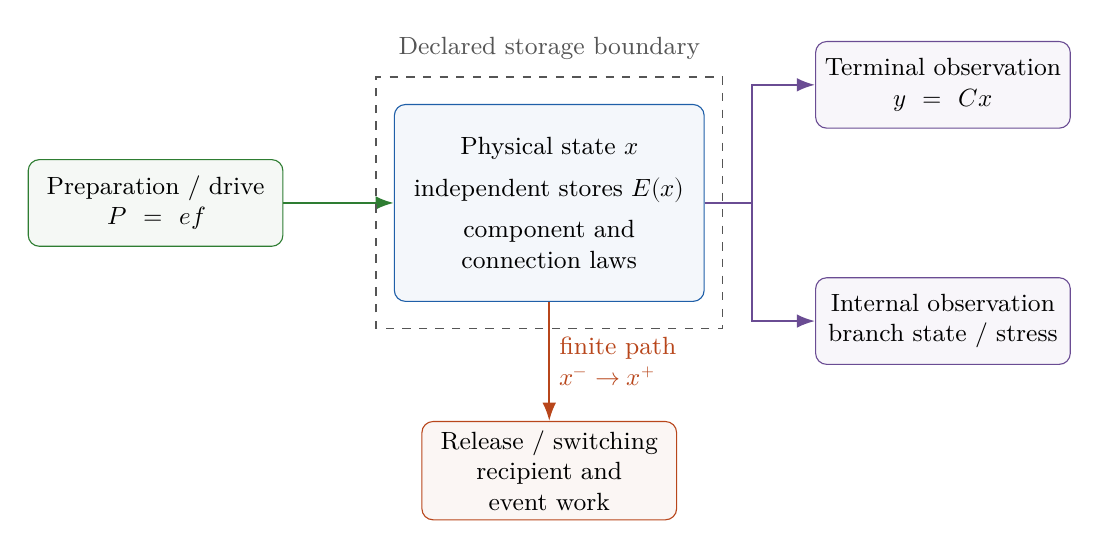
\begin{tikzpicture}[>=Latex,font=\small,
 box/.style={draw,rounded corners,align=center,minimum height=1.1cm,text width=3cm}]
\node[box,draw=elemA,fill=elemA!5,text width=3.7cm,minimum height=2.5cm] (state) at (0,0)
 {Physical state $x$\\[4pt] independent stores $E(x)$\\[4pt] component and connection laws};
\node[box,draw=elemC,fill=elemC!5] (prep) at (-5,0) {Preparation / drive\\ $P=e f$};
\node[box,draw=elemD,fill=elemD!5] (obs) at (5,1.5) {Terminal observation\\ $y=Cx$};
\node[box,draw=elemD,fill=elemD!5] (inside) at (5,-1.5) {Internal observation\\ branch state / stress};
\node[box,draw=elemB,fill=elemB!5] (release) at (0,-3.4) {Release / switching\\ recipient and event work};
\draw[->,thick,elemC] (prep) -- (state);
\draw[->,thick,elemD] (state.east) -- ++(.6,0) |- (obs.west);
\draw[->,thick,elemD] (state.east) -- ++(.6,0) |- (inside.west);
\draw[->,thick,elemB] (state) -- node[right,align=left] {finite path\\ $x^-\to x^+$} (release);
\draw[dashed,frameline] (-2.2,-1.6) rectangle (2.2,1.6);
\node[frameline,anchor=south] at (0,1.7) {Declared storage boundary};
\end{tikzpicture}
\end{document}
